\chapter{Marco te\'orico}
\label{Chapter2}

En este capítulo se presenta una visión general de la bibliografía relacionada al objetivo del presente trabajo. En la
primera sección se detalla una revisión de trabajos relacionados. En ... % TODO: completar

\section{Reconocimiento de d\'igitos}
\lipsum[1]

\section{Redes Neuronales}
\lipsum[1]

\subsection{Redes densas}
\lipsum[1]
% TODO: hablar de pre-train y fine-tuning

\subsection{Convolucionales}
\lipsum[1]

\subsection{Arquitecturas}
\lipsum[1]

\subsubsection{LeNet}
\lipsum[1]

\subsubsection{ResNet}
\lipsum[1]

\section{Adaptaci\'on de Dominio}
El {\it pre-entrenamiento} y el {\it fine-tuning} han mejorado considerablemente el estado del arte para diversos
problemas y aplicaciones del machine learning, incluso las redes profundas pre-entrenadas pueden adaptarse fácilmente a
tareas donde se cuenta con una pequeña cantidad de datos etiquetados. Sin embargo, en muchos escenarios prácticos, no
hay datos de entrenamiento etiquetados y, por lo tanto, existe la necesidad de transferir el aprendizaje de una red
profunda desde un dominio de origen en el que se dispone de datos de entrenamiento etiquetados a un dominio de destino
en el que solo existen datos sin etiquetar \parencite{glorot2011domain}. En esta situación, los modelos profundos siguen sufriendo degradaciones de rendimiento debido
al cambio de distribución \parencite{quinonero2008dataset}. Por lo tanto, se propone la {\it adaptación de dominio} para reducir el cambio de
distribución entre los dominios de entrenamiento y de prueba \parencite{jiang2022machine}.

Se han propuesto muchos métodos para la adaptación de dominios, ya sea ponderando o seleccionando muestras del dominio
de origen \parencite{sugiyama2007direct} o buscando una transformación de la distribución de origen a la distribución de destino \parencite{gong2013connecting}. Esta tesis analizar\'a algunos de los m\'etodos m\'as actuales del ultimo caso.

\subsection{Domain Adversarial Neural Network}
Un gran hito al momento de modelar distribuciones es la Red Generativa Adversaria {\it GAN} \parencite{goodfellow2020generative}. Inspirada en estas arquitecturas GAN, la Red Neural Adversaria de Dominio {\it DANN} \parencite{ganin2016domain} dos redes en la adaptación del dominio (figura \ref{fig:esquema-dann}). La primera es la
discriminadora de dominios $\mathcal{D}$ entrenada para distinguir las características de origen de las de destino y la
segunda es a generadora de características $\mathcal{G}$ que se entrena para confundir a $\mathcal{D}$ y para ayudar a
la red clasificadora $\mathcal{C}$.

\begin{figure}[H]
    \centering

    \tikzset{every picture/.style={line width=0.75pt}} %set default line width to 0.75pt        

    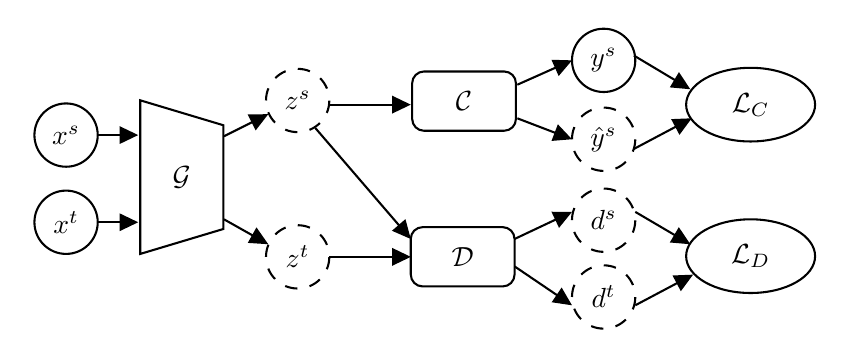
\begin{tikzpicture}[x=0.75pt,y=0.75pt,yscale=-1,xscale=1]
        \draw   (39,64.75) .. controls (39,56.33) and (45.83,49.5) .. (54.25,49.5) .. controls (62.67,49.5) and (69.5,56.33) .. (69.5,64.75) .. controls (69.5,73.17) and (62.67,80) .. (54.25,80) .. controls (45.83,80) and (39,73.17) .. (39,64.75) -- cycle ;

        \draw   (39,106.75) .. controls (39,98.33) and (45.83,91.5) .. (54.25,91.5) .. controls (62.67,91.5) and (69.5,98.33) .. (69.5,106.75) .. controls (69.5,115.17) and (62.67,122) .. (54.25,122) .. controls (45.83,122) and (39,115.17) .. (39,106.75) -- cycle ;

        \draw   (90,48) -- (130,60) -- (130,110) -- (90,122) -- cycle ;

        \draw    (69.5,64.75) -- (86,64.75) ;
        \draw [shift={(89,64.75)}, rotate = 180] [fill={rgb, 255:red, 0; green, 0; blue, 0 }  ][line width=0.08]  [draw opacity=0] (8.93,-4.29) -- (0,0) -- (8.93,4.29) -- cycle    ;
        \draw  [dash pattern={on 4.5pt off 4.5pt}] (150.58,48.08) .. controls (150.58,39.66) and (157.41,32.83) .. (165.83,32.83) .. controls (174.26,32.83) and (181.08,39.66) .. (181.08,48.08) .. controls (181.08,56.51) and (174.26,63.33) .. (165.83,63.33) .. controls (157.41,63.33) and (150.58,56.51) .. (150.58,48.08) -- cycle ;

        \draw  [dash pattern={on 4.5pt off 4.5pt}] (150.58,123.42) .. controls (150.58,114.99) and (157.41,108.17) .. (165.83,108.17) .. controls (174.26,108.17) and (181.08,114.99) .. (181.08,123.42) .. controls (181.08,131.84) and (174.26,138.67) .. (165.83,138.67) .. controls (157.41,138.67) and (150.58,131.84) .. (150.58,123.42) -- cycle ;

        \draw   (221,39.81) .. controls (221,36.65) and (223.56,34.1) .. (226.71,34.1) -- (265.29,34.1) .. controls (268.44,34.1) and (271,36.65) .. (271,39.81) -- (271,56.95) .. controls (271,60.11) and (268.44,62.67) .. (265.29,62.67) -- (226.71,62.67) .. controls (223.56,62.67) and (221,60.11) .. (221,56.95) -- cycle ;

        \draw   (220.33,114.81) .. controls (220.33,111.65) and (222.89,109.1) .. (226.05,109.1) -- (264.62,109.1) .. controls (267.77,109.1) and (270.33,111.65) .. (270.33,114.81) -- (270.33,131.95) .. controls (270.33,135.11) and (267.77,137.67) .. (264.62,137.67) -- (226.05,137.67) .. controls (222.89,137.67) and (220.33,135.11) .. (220.33,131.95) -- cycle ;

        \draw  [dash pattern={on 4.5pt off 4.5pt}] (298,105.75) .. controls (298,97.33) and (304.83,90.5) .. (313.25,90.5) .. controls (321.67,90.5) and (328.5,97.33) .. (328.5,105.75) .. controls (328.5,114.17) and (321.67,121) .. (313.25,121) .. controls (304.83,121) and (298,114.17) .. (298,105.75) -- cycle ;

        \draw  [dash pattern={on 4.5pt off 4.5pt}] (298,142.75) .. controls (298,134.33) and (304.83,127.5) .. (313.25,127.5) .. controls (321.67,127.5) and (328.5,134.33) .. (328.5,142.75) .. controls (328.5,151.17) and (321.67,158) .. (313.25,158) .. controls (304.83,158) and (298,151.17) .. (298,142.75) -- cycle ;

        \draw   (353,123.08) .. controls (353,113.28) and (366.91,105.33) .. (384.06,105.33) .. controls (401.22,105.33) and (415.13,113.28) .. (415.13,123.08) .. controls (415.13,132.89) and (401.22,140.83) .. (384.06,140.83) .. controls (366.91,140.83) and (353,132.89) .. (353,123.08) -- cycle ;

        \draw   (298,28.75) .. controls (298,20.33) and (304.83,13.5) .. (313.25,13.5) .. controls (321.67,13.5) and (328.5,20.33) .. (328.5,28.75) .. controls (328.5,37.17) and (321.67,44) .. (313.25,44) .. controls (304.83,44) and (298,37.17) .. (298,28.75) -- cycle ;
        \draw  [dash pattern={on 4.5pt off 4.5pt}] (298,66.75) .. controls (298,58.33) and (304.83,51.5) .. (313.25,51.5) .. controls (321.67,51.5) and (328.5,58.33) .. (328.5,66.75) .. controls (328.5,75.17) and (321.67,82) .. (313.25,82) .. controls (304.83,82) and (298,75.17) .. (298,66.75) -- cycle ;
        \draw   (353,50.08) .. controls (353,40.28) and (366.91,32.33) .. (384.06,32.33) .. controls (401.22,32.33) and (415.13,40.28) .. (415.13,50.08) .. controls (415.13,59.89) and (401.22,67.83) .. (384.06,67.83) .. controls (366.91,67.83) and (353,59.89) .. (353,50.08) -- cycle ;
        \draw    (69.5,106.75) -- (86,106.75) ;
        \draw [shift={(89,106.75)}, rotate = 180] [fill={rgb, 255:red, 0; green, 0; blue, 0 }  ][line width=0.08]  [draw opacity=0] (8.93,-4.29) -- (0,0) -- (8.93,4.29) -- cycle    ;
        \draw    (130.33,65.33) -- (148.98,56.01) ;
        \draw [shift={(151.67,54.67)}, rotate = 153.43] [fill={rgb, 255:red, 0; green, 0; blue, 0 }  ][line width=0.08]  [draw opacity=0] (8.93,-4.29) -- (0,0) -- (8.93,4.29) -- cycle    ;
        \draw    (130.33,105.33) -- (149.05,115.86) ;
        \draw [shift={(151.67,117.33)}, rotate = 209.36] [fill={rgb, 255:red, 0; green, 0; blue, 0 }  ][line width=0.08]  [draw opacity=0] (8.93,-4.29) -- (0,0) -- (8.93,4.29) -- cycle    ;
        \draw    (181.08,50.08) -- (217.33,50.08) ;
        \draw [shift={(220.33,50.08)}, rotate = 180] [fill={rgb, 255:red, 0; green, 0; blue, 0 }  ][line width=0.08]  [draw opacity=0] (8.93,-4.29) -- (0,0) -- (8.93,4.29) -- cycle    ;
        \draw    (181.08,123.42) -- (217.33,123.42) ;
        \draw [shift={(220.33,123.42)}, rotate = 180] [fill={rgb, 255:red, 0; green, 0; blue, 0 }  ][line width=0.08]  [draw opacity=0] (8.93,-4.29) -- (0,0) -- (8.93,4.29) -- cycle    ;
        \draw    (174.33,61.33) -- (218.38,112.54) ;
        \draw [shift={(220.33,114.81)}, rotate = 229.3] [fill={rgb, 255:red, 0; green, 0; blue, 0 }  ][line width=0.08]  [draw opacity=0] (8.93,-4.29) -- (0,0) -- (8.93,4.29) -- cycle    ;
        \draw    (270.33,114.81) -- (295.29,103.03) ;
        \draw [shift={(298,101.75)}, rotate = 154.73] [fill={rgb, 255:red, 0; green, 0; blue, 0 }  ][line width=0.08]  [draw opacity=0] (8.93,-4.29) -- (0,0) -- (8.93,4.29) -- cycle    ;
        \draw    (270.33,128) -- (295.52,145.07) ;
        \draw [shift={(298,146.75)}, rotate = 214.13] [fill={rgb, 255:red, 0; green, 0; blue, 0 }  ][line width=0.08]  [draw opacity=0] (8.93,-4.29) -- (0,0) -- (8.93,4.29) -- cycle    ;
        \draw    (328.5,101.75) -- (352.41,115.81) ;
        \draw [shift={(355,117.33)}, rotate = 210.46] [fill={rgb, 255:red, 0; green, 0; blue, 0 }  ][line width=0.08]  [draw opacity=0] (8.93,-4.29) -- (0,0) -- (8.93,4.29) -- cycle    ;
        \draw    (328.5,146.75) -- (353.68,133.4) ;
        \draw [shift={(356.33,132)}, rotate = 152.08] [fill={rgb, 255:red, 0; green, 0; blue, 0 }  ][line width=0.08]  [draw opacity=0] (8.93,-4.29) -- (0,0) -- (8.93,4.29) -- cycle    ;
        \draw    (271.67,40.48) -- (295.26,29.97) ;
        \draw [shift={(298,28.75)}, rotate = 156] [fill={rgb, 255:red, 0; green, 0; blue, 0 }  ][line width=0.08]  [draw opacity=0] (8.93,-4.29) -- (0,0) -- (8.93,4.29) -- cycle    ;
        \draw    (271.67,56.67) -- (295.2,65.68) ;
        \draw [shift={(298,66.75)}, rotate = 200.95] [fill={rgb, 255:red, 0; green, 0; blue, 0 }  ][line width=0.08]  [draw opacity=0] (8.93,-4.29) -- (0,0) -- (8.93,4.29) -- cycle    ;
        \draw    (327.83,26.42) -- (352.43,41.13) ;
        \draw [shift={(355,42.67)}, rotate = 210.89] [fill={rgb, 255:red, 0; green, 0; blue, 0 }  ][line width=0.08]  [draw opacity=0] (8.93,-4.29) -- (0,0) -- (8.93,4.29) -- cycle    ;
        \draw    (327.83,71.42) -- (353.02,58.07) ;
        \draw [shift={(355.67,56.67)}, rotate = 152.08] [fill={rgb, 255:red, 0; green, 0; blue, 0 }  ][line width=0.08]  [draw opacity=0] (8.93,-4.29) -- (0,0) -- (8.93,4.29) -- cycle    ;

        \draw (165.83,123.42) node   [align=left] {\begin{minipage}[lt]{21.08pt}\setlength\topsep{0pt}
                \begin{center}
                    $z^t$
                \end{center}

            \end{minipage}};
        \draw (165.83,48.08) node   [align=left] {\begin{minipage}[lt]{21.08pt}\setlength\topsep{0pt}
                \begin{center}
                    $z^s$
                \end{center}

            \end{minipage}};
        \draw (245.33,123.56) node   [align=left] {\begin{minipage}[lt]{26.23pt}\setlength\topsep{0pt}
                \begin{center}
                    $\mathcal{D}$
                \end{center}

            \end{minipage}};
        \draw (246,48.56) node   [align=left] {\begin{minipage}[lt]{26.23pt}\setlength\topsep{0pt}
                \begin{center}
                    $\mathcal{C}$
                \end{center}

            \end{minipage}};
        \draw (110,85) node   [align=left] {\begin{minipage}[lt]{22.78pt}\setlength\topsep{0pt}
                \begin{center}
                    $\mathcal{G}$
                \end{center}

            \end{minipage}};
        \draw (54.25,106.75) node   [align=left] {\begin{minipage}[lt]{21.08pt}\setlength\topsep{0pt}
                \begin{center}
                    $x^t$
                \end{center}

            \end{minipage}};
        \draw (54.25,64.75) node   [align=left] {\begin{minipage}[lt]{21.08pt}\setlength\topsep{0pt}
                \begin{center}
                    $x^s$
                \end{center}

            \end{minipage}};
        \draw (313.25,142.75) node   [align=left] {\begin{minipage}[lt]{21.08pt}\setlength\topsep{0pt}
                \begin{center}
                    $d^t$
                \end{center}

            \end{minipage}};
        \draw (313.25,105.75) node   [align=left] {\begin{minipage}[lt]{21.08pt}\setlength\topsep{0pt}
                \begin{center}
                    $d^s$
                \end{center}

            \end{minipage}};
        \draw (384.06,123.08) node   [align=left] {\begin{minipage}[lt]{32.64pt}\setlength\topsep{0pt}
                \begin{center}
                    $\mathcal{L}_D$
                \end{center}

            \end{minipage}};
        \draw (313.25,28.75) node   [align=left] {\begin{minipage}[lt]{21.08pt}\setlength\topsep{0pt}
                \begin{center}
                    $y^s$
                \end{center}

            \end{minipage}};
        \draw (313.25,66.75) node   [align=left] {\begin{minipage}[lt]{21.08pt}\setlength\topsep{0pt}
                \begin{center}
                    $\hat{y}^s$
                \end{center}

            \end{minipage}};
        \draw (384.06,50.08) node   [align=left] {\begin{minipage}[lt]{32.64pt}\setlength\topsep{0pt}
                \begin{center}
                    $\mathcal{L}_C$
                \end{center}
            \end{minipage}};
    \end{tikzpicture}

    \caption{Esquema de las {\it DANN}. Los supra indices $s$ y $t$ indican si los datos son del origen o destino respectivamente.
        Los c\'irculos con l\'ineas rayadas son salidas de los modelos mientras que los c\'irculos de l\'ineas s\'olidas son datos conocidos.}
    \label{fig:esquema-dann}
\end{figure}

Las redes DANN poseen una funci\'on de p\'erdida $\mathcal{L}$ que depende de $\mathcal{L}_\mathcal{C}$ y
$\mathcal{L}_\mathcal{D}$.

$\mathcal{L}_\mathcal{C}$ mide el error que posee la red en la clasificaci\'on de los datos de origen y viene dada por el {\it cross-entropy} $\mathcal{L}_{CE}$ aplicado a la salida de la red $\mathcal{C}$.

\begin{align}
    \mathcal{L}_\mathcal{C}(x^s, y^s) & = \mathcal{L}_{CE}(C(\mathcal{G}(x^s)), y^s) \nonumber                \\
                                      & = \mathcal{L}_{CE}(C(z^s), y^s) \nonumber                             \\
                                      & = \mathcal{L}_{CE}(\hat{y}^s, y^s) \label{eq:dann-loss-clasificadora}
\end{align}

La funci\'on de p\'erdida de $\mathcal{D}$ viene dada por la ecuaci\'on \ref{eq:dann-loss-discriminadora}, donde
$\mathbb{E}_{x^s \sim \mathcal{\hat{S}}}$ y $\mathbb{E}_{x^t \sim \mathcal{\hat{T}}}$ representan la proporci\'on
esperada de datos de origen $\mathcal{\hat{S}}$ y destino $\mathcal{\hat{T}}$ respectivamente.

\begin{align}
    \mathcal{L}_\mathcal{D}(x^s, x^t) & = \mathbb{E}_{x^s \sim \mathcal{\hat{S}}}\log[\mathcal{D}(\mathcal{G}(x^s))] + \mathbb{E}_{x^t \sim \mathcal{\hat{T}}}\log[1-\mathcal{D}(\mathcal{G}(x^t))] \nonumber \\
                                      & = \mathbb{E}_{x^s \sim \mathcal{\hat{S}}}\log[\mathcal{D}(z^s)] + \mathbb{E}_{x^t \sim \mathcal{\hat{T}}}\log[1-\mathcal{D}(z^t)] \nonumber                           \\
                                      & = \mathbb{E}_{x^s \sim \mathcal{\hat{S}}}\log[d^s] + \mathbb{E}_{x^t \sim \mathcal{\hat{T}}}\log[1-d^t] \label{eq:dann-loss-discriminadora}
\end{align}

Por lo tanto, el $\mathcal{L}$ de una {\it DANN} viene dado por la ecuaci\'on \ref{eq:dann-loss}. Donde $\lambda$ es un
hiper-par\'ametro a optimizar que regula el trade-off de la clasificaci\'on y la discriminaci\'on.

\begin{align}
    \mathcal{L}(x^s, x^t) = \mathcal{L}_\mathcal{C}(x^s, y^s) + \lambda \mathcal{L}_\mathcal{D}(x^s, x^t)
    \label{eq:dann-loss}
\end{align}

\subsection{AFN}
\lipsum[1]

\subsection{ADDA}
\lipsum[1]

\subsection{MDD}
\lipsum[1]

